\documentclass[10pt, a4paper]{beamer}
\usetheme{Berkeley}
\usecolortheme{sidebartab}

\begin{document}
	\setbeamertemplate{sidebar left}{}
	\title{Progress Presentation-I}
	\subtitle{e-Yantra Summer Internship-2018 \\ $ \textbf{Low Cost Sensor Node} $}
	\author{Sachin Jadhav\\Nithin Thilakappan\\Nishit Patel\\ \vspace{1em}
	Mentors: \\ Parin Chheda, Kalind Karia}
	\institute{IIT Bombay}
	\date{\today}
	%\addtobeamertemplate{sidebar left}{}{\includegraphics[scale = 0.3]{logowithtext.png}}
	\frame{\titlepage}

\setbeamertemplate{caption}[numbered]
\setbeamertemplate{sidebar left}[sidebar theme]
\section{Overview of Project}
\begin{frame}{Overview of Project}
	\begin{itemize}
		\item \textcolor{blue}{Project Name:} Low Cost Sensor Node
		\item \textcolor{blue}{Objectives:}
        	\begin{enumerate}
        		\item A custom built power supply for optimized for low power sensor node applications
				\item Ability to program via Arduino IDE/ Atmel Studio
				\item Use nRF2401 for RF communication
				\item Completely open source design and sample codes to make it useful for WSNs
				\item Can be used as general purpose microcontroller board for learning interfacing and C
programming
                \end{enumerate}
		\item \textcolor{blue}{Deliverables:}
        \begin{enumerate}
        		\item A sensor node platform along with sample codes for rapid prototyping
				\item A firmware for low power modes and nRF24L01 networking
				\item Documenation on Hardware and Software
			
                \end{enumerate} 
	\end{itemize}
\end{frame}

\section{Overview of Task}
\begin{frame}{Overview of Task}
	\begin{table}
    \resizebox{\textwidth}{!}{
    \begin{tabular}{| c | p{23em} | c |}\hline
    	\textbf{Task No.} & \centering\textbf{Tasks} & \textbf{Completion}  \\\hline
    	1 &\small{Study about different sensor nodes platform available and their USP. Take desirable aspects of each} & Completed \\\hline
        2 &\small{Review low power modes in ATmega328p, nRF2401 literature review} & Completed \\\hline
        3 &\small{Build prototype using Arduino Pro Mini and nRF2401, test range theoretically and experimentally in outdoor environment} & Completed \\\hline
        4 &\small{Research components available and select to fit price v/s performance metric} & Completed \\\hline
        5 &\small{Build PCB design, source components, evaluation in Proteus (if necessary)} & Completed \\\hline
        6 &\small{Prototype soldering and testing} & Pending \\\hline
        7 &\small{Building a network of 3 nodes, relaying info, power consumption analysis} & Working on \\\hline
        8 &\small{Making reusable firmware for nRF2401, interfacing soil moisture, temperature/humidity sensors} & Working on \\\hline
        9 &\small{Gateway implementation using ESP32} & Completed \\\hline
        10 &\small{Firmware documentation, hardware manual and reporting result} & 3 \\\hline
    \end{tabular}}
    \end{table}
  \label{tab:addlabel}
!\end{frame}



\section{Task Accomplished}
\begin{frame}{Task Accomplished}
	\begin{itemize}
		\item  Change fuse bit in Atmega328p as per our application
        \item Complete circuit designing and send to printing
         \item Writing SPI library for Atmega328p in Atmel Studio
    	 \item Replacing Arduino core functions with our own GPIO functions for Atmega328p
         \item Testing of nRF24L01 transceiver on new firmware for our WSN 
     	 \item Implement mesh and star network using 3 nodes
         \item Complete Duty cycling of Atmega328p
 \end{itemize}

\end{frame}


\begin{frame}{Task Accomplished}
\begin{figure}
\begin{center}
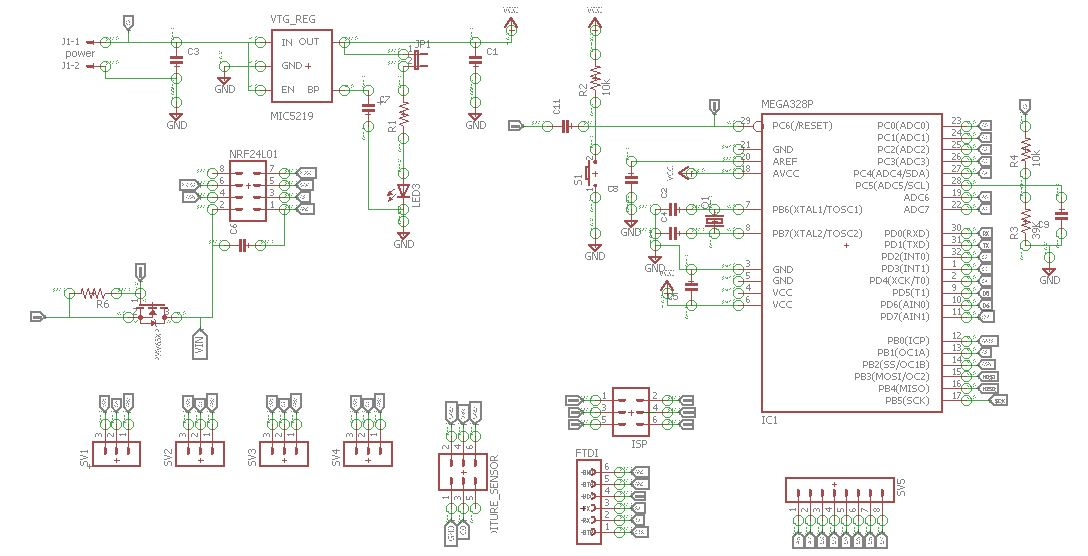
\includegraphics[width=1\textwidth]{eagle_sch_snap.JPG}
\caption{Schematic Design}
\end{center}
\end{figure}
\end {frame}

\begin{frame}{Task Accomplished}
\begin{figure}
\begin{center}
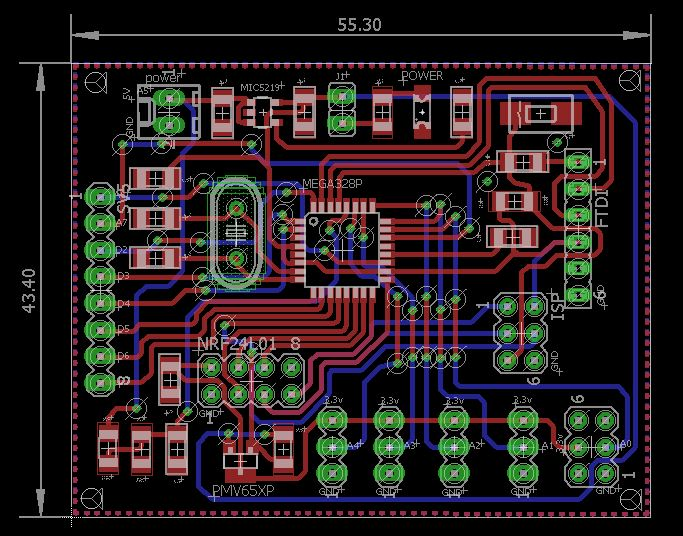
\includegraphics[width=0.8\textwidth]{eagle_board_snap.JPG}
\caption{Board Design}
\end{center}
\end{figure}
\end {frame}

\begin{frame}{Task Accomplished}
\begin{figure}
\begin{center}
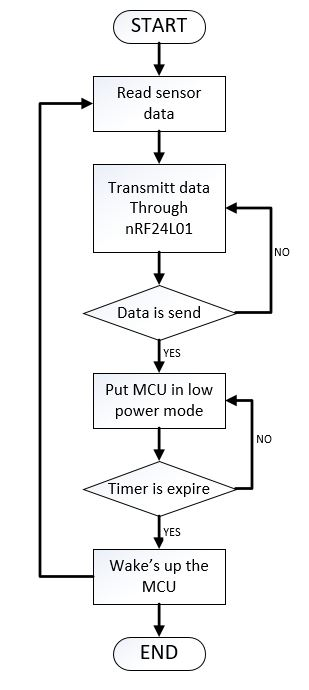
\includegraphics[width=0.25\textwidth]{trance_flow_snap.JPG}
\caption{Transmitter flow}
\end{center}
\end{figure}
\end {frame}

\begin{frame}{Task Accomplished}
\begin{figure}
\begin{center}
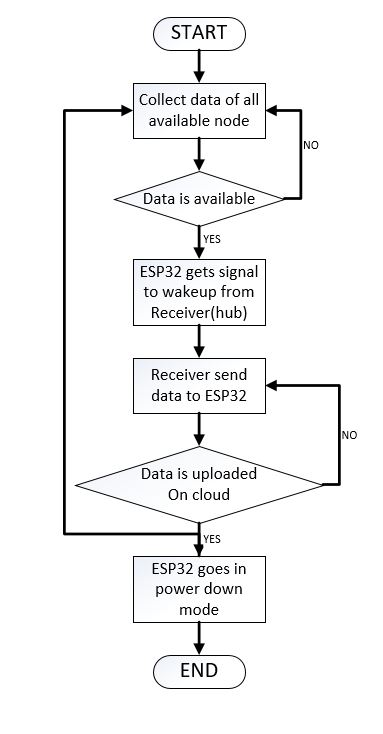
\includegraphics[width=0.3\textwidth]{receiver_flow_snap.JPG}
\caption{Receiver flow}
\end{center}
\end{figure}
\end {frame}


\begin{frame}{Task Accomplished}
\begin{figure}
\begin{center}
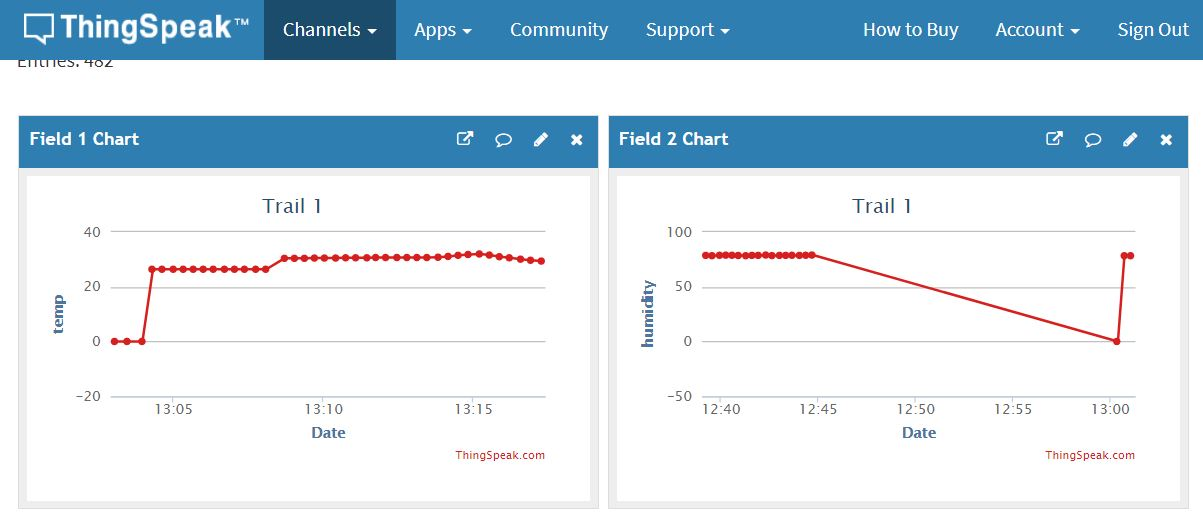
\includegraphics[width=1\textwidth]{graph_thingspeak.JPG}
\caption{Graph of uploaded data}
\end{center}
\end{figure}
\end {frame}


\section{Challenges Faced}
\begin{frame}{Challenges Faced}
	\begin{itemize}
		\item Importing C file in C++ ATMEL project.
        \item Understanding new concept in embedded C++
        \item Timing issue with SPI library
        \item Transmit and Receive flot value in string 
        \item Synchronization in Star network with duty cycling on both sides
	\end{itemize} 
\end{frame}



\section{Future Plans}
\begin{frame}{Future Plans}
	\begin{itemize}
		\item PCB soldering and testing
        \item Setup of 5 nodes WSN star network
        \item Operating life prediction of WSN
        \item Add soil moisture, light intensity sensor, humidity sensor on board and make provision to connect other sensors if needed
        \item Improvement in receiver for gateway implementation
	\end{itemize}
\end{frame}


\section{Thank You}
\begin{frame}{Thank You}
	\centering THANK YOU !!!
\end{frame}
\end{document}